\section{One saddle expansion throughout the harmonic-depth range}
\label{cont26:sec:uniform}

The source manuscript proves separate expansions when $p/h$ lies in a
fixed compact interval, when $p/h=\log h+c$, and when $p$ is fixed.
It explicitly leaves a uniform connection between the first two regimes
open \cite{ProveIt}. We supply that connection and a larger parameter
range. The central point is to keep the shift $a$ in the saddle equation
and to use $p$ as the expansion parameter.

\subsection{The sum and its positive integral}
For an integer $h\geq1$ put
\[
 e_h(n)=[u^h]\prod_{j=1}^n(1+u/j),\qquad
 T_{p,h}(a)=\sum_{n=0}^{\infty}\frac{(-1)^n e_h(n)}{(n+a)^p},
 \qquad p,a>0.
\]
The ordinary sum converges for every $p>0$; for $p>1$ it converges
absolutely. To see the former claim directly, the elementary-symmetric
function bound $e_h(n)\leq H_n^h/h!$ gives decay of the terms, and
$e_h(n+1)-e_h(n)=e_{h-1}(n)/(n+1)$ gives eventual decrease of
$e_h(n)/(n+a)^p$. For example $e_h(n)\sim(\log n)^h/h!$, as follows
by expanding the fixed-degree coefficient in
$\exp(\sum_{j\geq1}(-1)^{j-1}H_n^{(j)}u^j/j)$.

Define the positive normalization
\begin{equation}\label{cont26:eq:R}
 R_{p,h}(a)=(-1)^h h!(h+a)^pT_{p,h}(a).
\end{equation}
The generating function
\[
 \sum_{n\geq0}e_h(n)z^n
 =\frac{(-\log(1-z))^h}{h!(1-z)}
\]
and the gamma integral give
\begin{equation}\label{cont26:eq:positive}
 R_{p,h}(a)=\frac{(h+a)^p}{\Gamma(p)}
 \int_0^{\infty}\frac{y^{p-1}e^{-ay}L(y)^h}{1+e^{-y}}\,dy,
 \qquad L(y)=\log(1+e^{-y}).
\end{equation}
One may insert a radial Abel factor before interchanging sums and
integrals, then use dominated convergence and the ordinary convergence
just established. This is the source manuscript's positive integral,
recalled here to make the continuation self-contained.

It is useful to set
\begin{equation}\label{cont26:eq:H-w}
 H(x)=\log(e^xL(x)),\qquad
 w(x)=-\frac{d}{dx}\log L(x)
 =\frac1{(1+e^x)L(x)}.
\end{equation}
Then $H'=1-w$, $H''=-w'<0$, and
\begin{equation}\label{cont26:eq:w-bound}
 w_0:=\frac1{2\log2}<w(x)<1,\qquad w'(x)>0.
\end{equation}
Indeed, with $t=e^{-x}$,
$w=t/((1+t)\log(1+t))$, whose logarithmic derivative with respect
to $t$ is $(\log(1+t)-t)/(t(1+t)\log(1+t))<0$.
The function $H$ extends smoothly to $x=0$; all of its positive-order
derivatives decay exponentially as $x\to\infty$.

\subsection{Exact saddle and main theorem}
There is exactly one $x=x(p,h,a)>0$ satisfying
\begin{equation}\label{cont26:eq:saddle}
 x\{h w(x)+a\}=p.
\end{equation}
The left side has a strictly positive derivative and runs from zero
to infinity. In particular,
\begin{equation}\label{cont26:eq:x-bracket}
 \frac{p}{h+a}<x<\frac{p}{h w_0+a}.
\end{equation}
Define
\begin{align}
 \theta&=\frac{hx}{p}=\frac{h}{h w(x)+a},&
 B&=1+\theta xw'(x),\label{cont26:eq:thetaB}\\
 \delta&=\frac{(h+a)x}{p}-1,&
 E&=p\{\log(1+\delta)-\delta\}+hH(x),\label{cont26:eq:E}\\
 \mathcal A(p,h,a)&=\frac{e^E}{(1+e^{-x})\sqrt B}.
 \label{cont26:eq:Auniform}
\end{align}
All these quantities are real. Both summands in $E$ are nonpositive,
which also makes \eqref{cont26:eq:E} a useful form for numerical evaluation.

\begin{theorem}[Uniform moving-saddle expansion]\label{cont26:thm:uniform}
For each integer $J\geq0$ there are bounded, explicitly computable
coefficient functions $d_j(x,\theta)$, $0\leq j\leq J$, with $d_0=1$,
and constants $C_J,p_J$ depending only on $J$, such that
\begin{equation}\label{cont26:eq:uniform-all}
 \left|\frac{R_{p,h}(a)}{\mathcal A(p,h,a)}
       -\sum_{j=0}^J\frac{d_j(x,\theta)}{p^j}\right|
 \leq \frac{C_J}{p^{J+1}}
\end{equation}
for every real $p\geq p_J$, every integer $h\geq1$, and every $a>0$.
There is no lower or upper restriction on $p/h$, and $a$ may also vary.
The constants in the error bound are independent of all three parameters.
In particular, $R_{p,h}(a)=\mathcal A(p,h,a)(1+O(p^{-1}))$ uniformly.
\end{theorem}

Here is the first coefficient in a form that only uses derivatives at the
single real saddle. Write
\begin{align}
 v&=(1+e^x)^{-1},&
 \ell_1&=-1+xv,&\ell_2&=1-x^2v(1-v),\notag\\
 b_3&=2-\theta x^2w''(x),&
 b_4&=-6-\theta x^3w'''(x).\label{cont26:eq:first-data}
\end{align}
Then
\begin{equation}\label{cont26:eq:d1}
 d_1=\frac{\ell_2+\ell_1^2}{2B}
     +\frac{b_3\ell_1}{2B^2}
     +\frac{b_4}{8B^2}
     +\frac{5b_3^2}{24B^3}-\frac1{12}.
\end{equation}
The final $-1/12$ is the gamma-normalization correction. Omitting it
would fail even in the limiting pure-gamma model.

\begin{figure}[tbp]
\centering
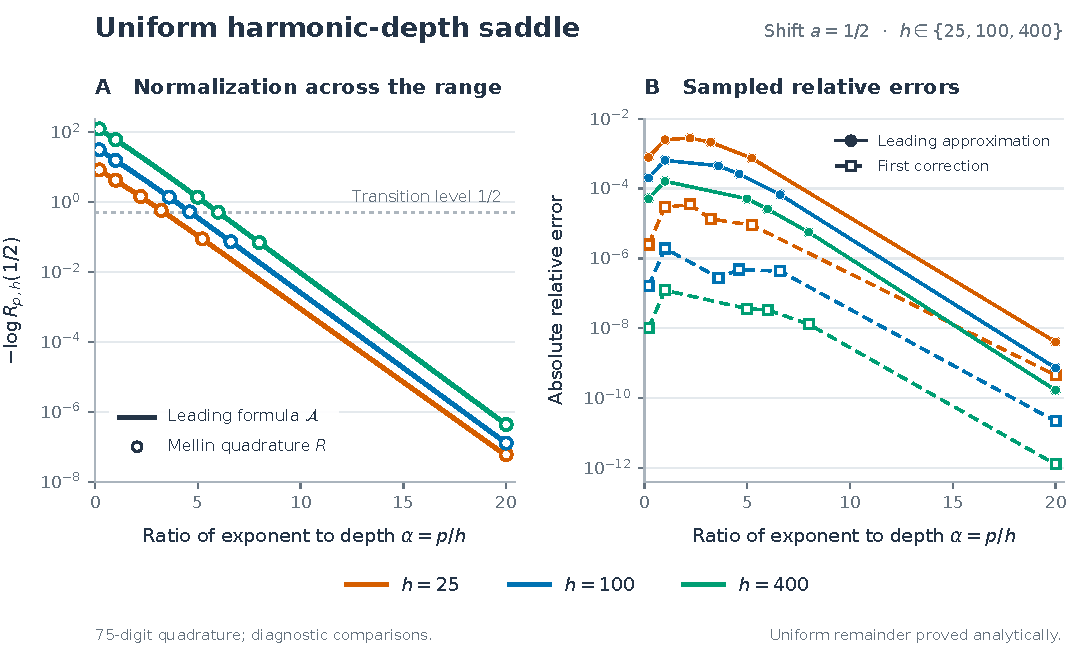
\includegraphics[width=\textwidth]{figures/uniform_harmonic_saddle.pdf}
\caption{Uniform harmonic-depth approximation at $a=1/2$, for
$h=25,100,400$. Both vertical axes are logarithmic.
\textbf{(A)} Solid curves show $-\log\mathcal A$ from the explicit
moving-saddle formula over $0.2\leq\alpha=p/h\leq20$; circles show
$-\log R$ from $75$-digit Mellin quadrature. The horizontal guide at
$1/2$ is the transition limit $-\log R_{h\log h,h}(1/2)\to1/2$.
\textbf{(B)} Absolute relative errors of the leading approximation
$\mathcal A$ and its first correction $\mathcal A(1+d_1/p)$ at the
$18$ sampled parameters. Connecting segments guide the eye.
These are numerical diagnostics; the analytic proof of
Theorem~\ref{cont26:thm:uniform} supplies the uniform remainder estimate.}
\label{cont26:fig:uniform-harmonic-saddle}
\end{figure}

\subsection{A uniform Laplace lemma and proof}
Put $y=xu$ in \eqref{cont26:eq:positive}. The phase and amplitude, normalized
at their unique saddle $u=1$, are
\begin{align}
 \phi(u)&=\log u-u+1+\frac{\theta}{x}
       \{H(xu)-H(x)-xH'(x)(u-1)\},\label{cont26:eq:phase}\\
 g_x(u)&=\frac1{u(1+e^{-xu})}.\label{cont26:eq:amp}
\end{align}
Thus $\phi(1)=\phi'(1)=0$, $-\phi''(1)=B$, and the exact integral is
\begin{equation}\label{cont26:eq:exact-scaled}
 R_{p,h}(a)=\frac{(h+a)^p x^p L(x)^h e^{-ax}}{\Gamma(p)}
             \int_0^\infty e^{p\phi(u)}g_x(u)\,du.
\end{equation}

The following four bounds hold uniformly in $x>0$ and
$0\leq\theta\leq1/w(x)$, a set containing every saddle parameter above.
\begin{enumerate}
\item Concavity of $H$ gives the global bound
\begin{equation}\label{cont26:eq:global-gamma-bound}
 \phi(u)\leq\log u-u+1\quad (u>0).
\end{equation}
\item The curvature is uniformly nondegenerate:
$1\leq B\leq1+w_0^{-1}\sup_{x>0}xw'(x)<\infty$.
\item On $1/2\leq u\leq3/2$, each fixed derivative of $\phi$ is
uniformly bounded. For $m\geq2$ the only extra term beyond a derivative
of $\log u-u+1$ is
$\theta x^{m-1}H^{(m)}(xu)$. Its boundedness follows from smoothness
at zero and exponential decay at infinity. Derivatives of $g_x$ are
uniformly bounded on the same interval, while
$1/2\leq g_x(1)\leq1$.
\item Globally $0<g_x(u)\leq1/u$.
\end{enumerate}

For completeness, these bounds suffice for a parameter-uniform Laplace
expansion, rather than merely a pointwise use of the method
\cite{DLMF23,TemmeUniform}. Choose a fixed $0<\eta<1/2$.
The contribution of $|u-1|\geq\eta$ is bounded by
\[
 \int_{|u-1|\geq\eta}\frac{e^{p(\log u-u+1)}}u\,du
 \leq C p^{-1/2}e^{-c_\eta p}.
\]
One direct proof divides the integral by
$e^p\Gamma(p)/p^p$ and applies the elementary exponential Markov
bound to a gamma random variable of shape $p$ and rate $p$.
The two tail exponents are
$1\pm\eta-1-\log(1\pm\eta)>0$.
This controls the unbounded domain and the singular factor $1/u$ at once.

On $|u-1|<\eta$, set $u=1+z/\sqrt p$. Taylor-expand the phase and
amplitude to a fixed order. Uniform derivative bounds give uniform
Taylor remainders. The inequality \eqref{cont26:eq:global-gamma-bound} supplies
a fixed Gaussian majorant in this neighborhood. Splitting further at
$|z|=p^\varepsilon$, with a sufficiently small fixed $\varepsilon>0$
for the chosen order, justifies expansion of the exponential with an
integrable polynomial-times-Gaussian remainder. Outside that smaller
interval the same majorant is smaller than every inverse power of $p$.
Odd powers integrate to zero on the symmetric neighborhood, and extending
each polynomial Gaussian integral to the whole real line changes it by
an exponentially small quantity. Expanding two additional orders when
necessary gives, for every fixed $J$,
\begin{equation}\label{cont26:eq:uniform-laplace}
 \int_0^\infty e^{p\phi(u)}g_x(u)\,du
 =g_x(1)\sqrt{\frac{2\pi}{pB}}
   \left\{\sum_{j=0}^J\frac{c_j(x,\theta)}{p^j}
                  +O_J(p^{-J-1})\right\}.
\end{equation}
Every division here is by a quantity uniformly bounded away from zero.
This also proves uniform boundedness of each $c_j$.

Let
$\Gamma^*(p)=\Gamma(p)/(\sqrt{2\pi}p^{p-1/2}e^{-p})$.
Substitution of \eqref{cont26:eq:uniform-laplace} into
\eqref{cont26:eq:exact-scaled} gives $\mathcal A/\Gamma^*(p)$ times the
bracketed expansion. The ordinary positive-real Stirling expansion,
with its remainder \cite{DLMF511}, now proves
Theorem~\ref{cont26:thm:uniform} by multiplication of two finite expansions.
The displayed $c_1=d_1+1/12$ is obtained from the Gaussian moments of
degrees two, four and six. This proves \eqref{cont26:eq:d1} as well.

\subsection{A finite coefficient compiler}
The proof specifies every coefficient without fitting any data. Let
$\phi_m=\phi^{(m)}(1)$ and $g_m=g_x^{(m)}(1)$.
For $j\geq0$ define the polynomial
\begin{equation}\label{cont26:eq:cj-polynomial}
 P_j(z)=[t^{2j}]
 \left(\sum_{r=0}^{2j}\frac{g_rz^rt^r}{r!}\right)
 \exp\left(\sum_{m=3}^{2j+2}\frac{\phi_mz^mt^{m-2}}{m!}\right).
\end{equation}
With the convention that odd Gaussian moments vanish,
\begin{equation}\label{cont26:eq:cj}
 c_j=\frac1{g_0}\sqrt{\frac B{2\pi}}
      \int_{\mathbb R}e^{-Bz^2/2}P_j(z)\,dz.
\end{equation}
The even moments are $(2r-1)!!B^{-r}$ after normalization.
Finally, as a formal power-series prescription,
\begin{equation}\label{cont26:eq:dj}
 \sum_{j\geq0}d_j\varepsilon^j
 =\exp\left(-\sum_{r\geq1}
 \frac{B_{2r}\varepsilon^{2r-1}}{2r(2r-1)}\right)
     \sum_{j\geq0}c_j\varepsilon^j.
\end{equation}
Only finitely many terms enter each coefficient. The expansion is an
asymptotic expansion; no convergence of \eqref{cont26:eq:dj} is asserted.

\subsection{Recovery of existing regimes and a new uniform connection}
For $a$ fixed and $p=\alpha h$ with $\alpha$ in a positive compact
interval, the new saddle solves
$x(w(x)+a/h)=\alpha$. Let $x_\alpha w(x_\alpha)=\alpha$ be the
source saddle. The implicit function theorem gives
\[
 x=x_\alpha-\frac{a x_\alpha}{h\{w(x_\alpha)+x_\alpha w'(x_\alpha)\}}
 +O(h^{-2}).
\]
The envelope derivative in $a/h$, or direct substitution, then gives
\begin{equation}\label{cont26:eq:old-recovery}
 \mathcal A(p,h,a)
 =C(\alpha,a)e^{-hI(\alpha)}(1+O(h^{-1})),
\end{equation}
where the source functions are
\[
 I(\alpha)=-\alpha\log(x_\alpha/\alpha)-\alpha-\log L(x_\alpha),
 \quad
 C(\alpha,a)=
 \frac{\sqrt{\alpha}}{\sqrt{\alpha+x_\alpha^2w'(x_\alpha)}}
 \frac{e^{a(\alpha-x_\alpha)}}{1+e^{-x_\alpha}}.
\]
The new result retains the actual saddle and therefore does not
expand a term whose error would grow with $\alpha$.

At the transition $p=h(\log h+c)$, $a,c$ in fixed compact sets,
write $\alpha=\log h+c$ and $\lambda=e^{-c}/2$.
Since $w(x)=1-e^{-x}/2+O(e^{-2x})$, the saddle has
$x=\alpha+O(\alpha/h)$, and consequently
\[
 hH(x)=-\lambda+O(\alpha/h),\qquad
 p\{\log(1+\delta)-\delta\}=O(\alpha/h),\qquad
 B=1+O(\alpha/h).
\]
It follows from the uniform theorem that
\[
 R_{p,h}(a)=e^{-\lambda}\{1+O(\alpha/h)\}.
\]
The source already proves a sharper transition expansion; the new
contribution is that the same unexpanded $\mathcal A$ has a uniform
relative error $O(1/p)$ across this transition and all intervening
values of $p/h$. Including $d_1/p$ improves it to $O(p^{-2})$.

For any fixed $\alpha_0>0$ and any function $M(h)\geq\alpha_0$,
Theorem~\ref{cont26:thm:uniform} gives, without an upper growth condition,
\begin{equation}\label{cont26:eq:expanding-range}
 \sup_{\substack{\alpha_0\leq p/h\leq M(h)\\a>0}}
 \left|\frac{R_{p,h}(a)}{\mathcal A(p,h,a)}-1\right|=O(h^{-1}).
\end{equation}
The corrected supremum is $O(h^{-2})$. This explicitly resolves the
expanding-range question in the proportional-depth chapter.

At $x\to\infty$, the phase tends to $\log u-u+1$, the amplitude
tends to $1/u$, and all $d_j$ for $j\geq1$ tend to zero. Thus the
gamma normalization is consistent with first-term dominance when also
$h e^{-x}\to0$, as happens for fixed $h$. The limit $x\to\infty$
alone does not imply $R\to1$ when the depth varies. Conversely,
the theorem also allows $p/h\to0$ provided $p\to\infty$; it makes
no claim about a bounded $p$, where a different endpoint expansion is
appropriate.

\subsection{Exact monotonicities}
The same positive representation gives useful checks on numerical work.
If $Y$ is gamma with shape $p$ and rate $h+a$, then
\[
 R_{p,h}(a)=\mathbb E\,k_h(Y),\qquad
 k_h(y)=\frac{(e^yL(y))^h}{1+e^{-y}}.
\]
The function $k_h$ is strictly increasing in $y$ and strictly decreasing
in $h$. Coupling gamma variables by addition proves that $R$ is strictly
increasing in $p$. Scaling a common gamma variable proves strict decrease
in $a$, and jointly increasing the rate and decreasing the kernel proves
strict decrease in the integer $h$ for fixed $p,a$. Also $0<R<1$.
These are exact statements, independent of an asymptotic regime.


